%%%%%%%%%%%%%%%%%%%%%%%%%%%%%%%%%%%%%%%%%
% University/School Laboratory Report
% LaTeX Template
% Version 3.1 (25/3/14)
%
% This template has been downloaded from:
% http://www.LaTeXTemplates.com
%
% Original author:
% Linux and Unix Users Group at Virginia Tech Wiki 
% (https://vtluug.org/wiki/Example_LaTeX_chem_lab_report)
%
% License:
% CC BY-NC-SA 3.0 (http://creativecommons.org/licenses/by-nc-sa/3.0/)
%
%%%%%%%%%%%%%%%%%%%%%%%%%%%%%%%%%%%%%%%%%

%----------------------------------------------------------------------------------------
%	PACKAGES AND DOCUMENT CONFIGURATIONS
%----------------------------------------------------------------------------------------

\documentclass{article}

\usepackage{graphicx} % Required for the inclusion of images
\usepackage{natbib} % Required to change bibliography style to APA
\usepackage{amsmath} % Required for some math elements 
\usepackage{amsthm}
\usepackage[hyphens]{url}
\usepackage{hyperref}
\usepackage{subcaption}
\usepackage{float}
\usepackage{array}
\usepackage{amssymb}

\usepackage{listings}

\setlength\parindent{0pt} % Removes all indentation from paragraphs

\newtheorem*{remark}{Theorem}
\newtheorem*{definition}{Definition}

%----------------------------------------------------------------------------------------
%	DOCUMENT INFORMATION
%----------------------------------------------------------------------------------------

\title{Homework \#6 \\Message Exchange Protocol Design \\[0.2em]\small{}CNS Course Sapienza} % Title and subtitle

\author{Riccardo \textsc{Prinzivalle}, 1904064} % Author name

\date{December 11, 2020} % Date for the report

\begin{document}

\maketitle % Insert the title, author and date

%----------------------------------------------------------------------------------------
%	SECTION 0
%----------------------------------------------------------------------------------------

\section{Homework Goal}

This homework contains a basic design and implementation of a message exchange \textit{secure} protocol. The idea is taken from different protocols learned from the slides and the lessons of the course. The implementation is done using the \textbf{Kathara} framework to virtualize a small network, while the protocol is written using bash scripting exploiting the \textbf{OpenSSL} library on Linux.

%----------------------------------------------------------------------------------------
%	SECTION 1
%----------------------------------------------------------------------------------------

\section{Protocol Design}

The protocol can be divided into three main functionalities: \textit{confidentiality}, \textit{message authentication} and \textit{entity authentication}. Each functionality is developed as follows:

\begin{itemize}
	\item \textbf{Confidentiality} is achieved by using symmetric encryption with AES in CBC mode with key length of 256 bits, which is the standard for confidentiality for NSA \cite{AES_NSA}, similar hint was found also here \cite{AES_stack}.
	\item \textbf{Message Authentication} is performed with SHA-256 using public key signature (OpenSSL supports directly HMAC but the version installed on the docker image on the background of Kathara is older than the minimum version implementing HMAC).
	\item \textbf{Entity Authentication} is based on a weaker version of the X.509 protocol, which introduces some vulnerabilities but simplifies the implementation, since this part is done by hand since OpenSSL contains only the primitives and not a complete authentication protocol. 
\end{itemize}

Let's analyze every part more in the details; weaknesses will be analyzed in section \ref{sec:secAn}.\newline
Encryption is the simpler; it is just based upon the primitive from OpenSSL, and it uses the primitive as follows: 

\begin{lstlisting}[breaklines]
	openssl aes-256-cbc -in message/to/encrypt -out encrypted/message.enc -pass file:key/file
\end{lstlisting}

The key used is based on a shared secret from a DH key exchange phase performed previously, and the secret is hashed in order to obtain the desired length of 256 bits for the encryption key. The instruction used is:

\begin{lstlisting}[breaklines]
	openssl dgst -sha256 -out hashed/key.sha256 shared/secret.bin
\end{lstlisting}

To decrypt the message, it is easy as the encryption, it is just necessary to have the shared secret, derive the key by using hashing (as seen upside) and then decrypt with the following command:

\begin{lstlisting}[breaklines]
	openssl aes-256-cbc -d -in encrypted/message.enc -out decrypted/message -pass file:key/file
\end{lstlisting}

As already said, OpenSSL implements different primitives for authenticating messages, the problem resides in the version shipped with the docker image used in the practical experiment: it is older, so it does not support these new addition to the library. Due to this inconvenience, I found \cite{signatures} that it is possible to use message digest with SHA256 with a public key pair for digital signature of a message using OpenSSL, the command is the following:

\begin{lstlisting}[breaklines]
	openssl dgst -sha256 -sign private/key.pem -out message/signature.sha256 encrypted/message.enc
\end{lstlisting}

Then both the encrypted message and its signature are sent to the recipient of the message.





%----------------------------------------------------------------------------------------
%	SECTION 3
%----------------------------------------------------------------------------------------

\section{Protocol Proof of Concept}

This work compares the proposed implementation of RSA with a common library implementation of RSA itself and AES, the last one just to have an idea of how symmetric ciphers are in general more computational efficient than asymmetric ones. To have a fair comparison, AES uses 128 bit key, so as stated in table \ref{tab:keyLen}, it is necessary to have 3072 bit key for RSA. In the implementation proposed, since the key must have a length of 3072 bit, both $p$ and $q$ have a length of 1536 bit so their product has the correct length for the resulting key, as stated in section 7.6 of \cite{10.5555/1721909}.

\renewcommand{\arraystretch}{2}

\begin{table}[H]
	\begin{center}
		\begin{tabular}{ |c || c | c | c | c | c | c | }
			\hline
			Algorithm Family & Cryptosystems & \multicolumn{4}{c |}{Security Level (bit)}\\
			& & 80 & 128 & 192 & 256\\ [0.5ex] 
			\hline\hline
			Integer Factorization & RSA & 1024 & 3072 & 7680 & 15360  \\ 
			
			Discrete Logarithm & DH, DSA, Elgamal & 1024 & 3072 & 7680 & 15360  \\ 
			
			Elliptic Curves & ECDH, ECDSA & 160 & 256 & 384 & 512  \\ 
			\hline
			Symmetric key & AES, 3DES &  80 & 128 & 192 & 256  \\ 
			\hline
		\end{tabular}
		\caption{Key length comparison in public key and symmetric key algorithm}
		\label{tab:keyLen}
	\end{center}
\end{table}

The 3072 bit key allows to encrypt a maximum of $3072 \div 8 = 384$ bytes, this is due to the characteristics of RSA itself, otherwise the modulo reduction will collapse the oversize message inside the modulo domain and it will be impossible to recover the original message after decryption. To overcome this limit, an idea could be to implement operation mode on asymmetric ciphers, but it is not feasible due to the fact that these ciphers are so much slower with respect to symmetric ones, and it is better to use the latter to encrypt larger messages. For these reasons, the message to be encrypted has been chosen of dimension around 313 bytes. The proposed implementation needs to preprocess data to be sure to give to the encryption phase a integer number, this is done by the instruction \verb+binarybuffer = ''.join(format(ord(x), 'b') for x in buffer)+ which \linebreak produces an output in binary form, which is then converted into base ten numbers by using the instruction \verb+int(binarybuffer, 2)+ whose output is used in the encryption phase.\newline
For \textbf{RSA} comparison, both the key generation and message encryption are measured separately; the key generation is called once for every test since it requires more time with respect to the encryption phase, while the message encryption can be called more times by specifying the number of rounds when calling the function. Since the key generation phase requires different time depending on the test performed, I decided to perform 4 times the tests in different times of the day, and the median value are represented in tab. \ref{tab:RSA}; encryption and decryption value are much more stable in different tests (All the original tests value can be found in the output.txt file attached with this report).

\renewcommand{\arraystretch}{2}

\begin{table}[H]
	\begin{center}
		\begin{tabular}{ |c || m{2cm} | m{2cm} | m{2cm}|  }
			\hline
			RSA & key \linebreak generation & encryption \linebreak throughput & decryption \linebreak throughput \\ [0.5ex] 
			\hline\hline
			PyCryptoDome & 11.68 sec & 52,7 KB/s & 6,37 KB/s \\ 
			\hline
			Proposed implementation & 6.73 sec & 0,825 KB/s & 0.807 KB/s \\ 
			\hline
		\end{tabular}
		\caption{RSA time and throughput comparison}
		\label{tab:RSA}
	\end{center}
\end{table}

It is necessary to add that \textit{PyCryptoDome} RSA implements a padding scheme, while the proposed implementation does not, which offer less security and maybe requires less computation effort. The strange thing is that the proposed key generation algorithm needs less time on average with respect to the \textit{PyCryptoDome} one: as stated in \cite{pyrandom}, os.urandom, which is used here to generate the prime random numbers, uses on windows (on which I performed the tests) the function CryptGenRandom \cite{winRandom}, which I was not able to understand if it waits effectively for the entropy pool to be full enough, but since os.urandom uses /dev/urandom on Linux machines, which does not check if the entropy pool is filled up, probably neither the windows function does it, so here the reason for which the proposed implementation needs less time on average.\newline  
Instead, as it was easily predictable, the library implementation has much more throughput, both in encryption and decryption, with slower decryption, while the proposed implementation has much more similar time for both phases (it uses the same function for both), probably the library implementation has some tricks to speed up the process which are possible only on one way in encryption.\newline
To obtain a comparison with AES, I have chosen to use the ECB mode with padding; this is just for educational purposes, it is already known that symmetric ciphers are faster than public keys ones. The comparison is represented in tab. \ref{tab:RSA}.

\begin{table}[h]
	\begin{center}
		\begin{tabular}{ | c || m{2cm} | m{2cm} | }
			\hline
			AES vs RSA & Encryption & Decryption \\ [0.5ex] 
			\hline\hline
			AES ECB mode & 1,49 MB/s & 1,49 MB/s  \\ 
			\hline
			Proposed RSA & 0,825 KB/s & 0.807 KB/s \\ 
			\hline
		\end{tabular}
		\caption{RSA vs AES comparison}
		\label{tab:AES}
	\end{center}
\end{table}

Here, the time used by the key generation phase in RSA is not represented since the comparison this time is just on the pure encryption and decryption phase assuming we already have the keys for both algorithms.

%----------------------------------------------------------------------------------------
%	SECTION 4
%----------------------------------------------------------------------------------------

\section{Security Analysis}
\label{sec:secAn}

\begin{figure}[H]
	\centering
	%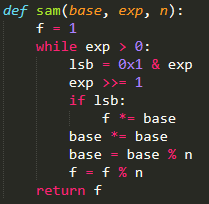
\includegraphics[width=0.345\linewidth]{images/SAM.png}
	\caption{Improved version of Square And Multiply}
	\label{fig:sam}
\end{figure}

%----------------------------------------------------------------------------------------
%	SECTION 5
%----------------------------------------------------------------------------------------

\section{Conclusion}

In this homework, as a difference with respect to the AES implementation, the code is based mainly on existent libraries, with the exception of few functions, whose implementation is based on pseudocode of already known algorithms, with small improvements in order to speed up the computations. The bigger improvement is the introduction of the modulo reduction on every computation of SAM, without it the proposed implementation didn't work as the result grew too much and it remained stuck after some iterations. As expected, also in this case the work is slower than the library implementation, with the exception of the key generation phase, which needs much more digging to reach the real cause of its larger throughput.

%----------------------------------------------------------------------------------------
%	BIBLIOGRAPHY
%----------------------------------------------------------------------------------------

\bibliographystyle{abbrv}

\bibliography{biblio}

%----------------------------------------------------------------------------------------


\end{document}